% 
% 
%			4: Algorithms
\chapter{Algorithms}
\label{chap:algorithms}

In market-basket analysis we are interested in the absolute number of baskets that contain a particular set of items.
The naive approach is to generate all the pairs for each basket using the double loop. But it may fail if there are too many pairs of items to count in main memory. 

In order to reduce the number pairs that must be counted special algorithms were designed. These algorithms are based on several passes over data and monotonicity if itemsets (if a set I of items is frequent, then so is every subset of I). 
In this work two algorithms are condisered: A-Priori and PCY.


\section{A-Priori}
The A-Priori Algorithm performs two passes over data:
\begin{enumerate}
	\item Count the occurences of each item in baskets - determine the \texttt{frequent items}; 
	\item Count all the pairs that consist of frequent items - \texttt{candidate pairs}; 
	\item Define the support threshold (typically 1\% of baskets) and analyse the resulting \texttt{frequent pairs}.
\end{enumerate}


The A-Priori algorithm is good enough when it has enough memory to count all the candidate pairs.
But in most cases the number of frequent pairs is very small, so the A-Priori algorithm uses unnecessary resources. In the case of considered dataset sample only 3\% of all pairs turned out to be frequent.


\section{PCY}
The PCY (Park, Chen and Yu) algorithm exploits the fact that A-Priori uses a lot of unnecessary resources to count of frequent singletons.
During the first pass the PCY algorithm not only counts each item occurences, but also generates pairs, hashes them to buckets and counts.
If the count of a bucket is at least as great as the support threshold, it is called a frequent bucket.

In order to implement PCY algorithm I made next changes to the A-Priori:
\begin{itemize}
	\item the algorithm will not generate all possible candidate pairs and loop through them with dataframe lookups;
	\item instead, it will go through each basket with frequent items and implement a bucket (=pair) counter while examining baskets.
\end{itemize}

In order to compare the two algorithms I have run both of them multiple times. The PCY's performance is times faster on average (~40 000 vs 8 microseconds):

\begin{itemize}
	\item A-Priori: 39.2 milliseconds ± 4.81 per loop (mean ± std. dev. of 7 runs, 3 loops each);
	\item PCY: 7.82 microseconds ± 4.52 per loop (mean ± std. dev. of 7 runs, 3 loops each).
\end{itemize}

The resulting sets of frequent pairs for both algorithms run on the full dataset showed no difference.
On average the A-Priori implementation needs 1700 millseconds to get frequent pairs from the full dataset, while the PCY implementation - less than 100 milliseconds. 

\section{Scaling}

The scaling of PCY implementation in terms of used memory was analysed. To do this the total memory used by objects in the enviroment was estimated for two cases: partial dataset and full dataset.

\begin{figure}[h]
	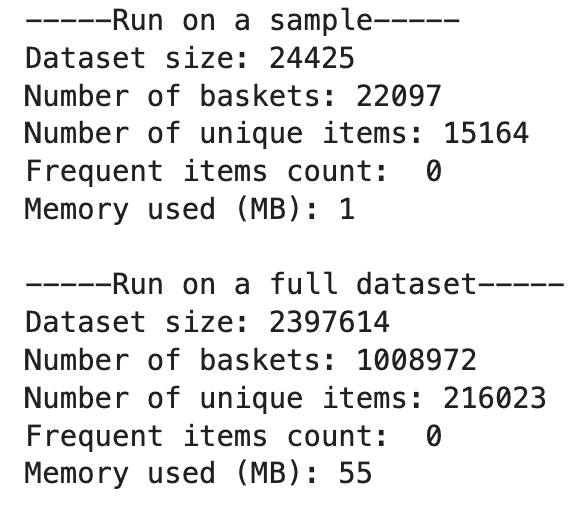
\includegraphics[width=6cm]{images/4-memory_tests}
\centering
\end{figure}

I would say that the PCY implementation scales well enough:
to process a 100 times larger dataset the we need 54 MB of RAM more.


